%%%%%%%%%%%%%%%%%%%%%%%%%%%%%%%%%%%%%%%%%%%%%%%%%%%%%%%%%%%%%%%%%%%%%%%%%%%
% Copyright (c) 2010 committers of YAKINDU and others.
% All rights reserved. This program and the accompanying materials
% are made available under the terms of the Eclipse Public License v1.0
% which accompanies this distribution, and is available at
% http://www.eclipse.org/legal/epl-v10.html
%
% Contributors:
%     committers of YAKINDU - initial API and implementation
%%%%%%%%%%%%%%%%%%%%%%%%%%%%%%%%%%%%%%%%%%%%%%%%%%%%%%%%%%%%%%%%%%%%%%%%%%%
\section{YAKINDU Statechart Tools}

YAKINDU is a tool kit for model based development and the statechart tools are
the first modules provided by this project. The tools apply the concept of
state machines that are well understood and formal enough to describe
behaviour unambiguously. The statechart tools support editing, validating,
simulating state machines and generating code from state machines. The tools
are provided as Eclipse-plugins and integrate tightly into the IDE.

The simulation of a state machine is integrated into the YAKINDU state machine
Diagram Editor and provides visual highlighting of the active state and the
current transition. Additionally, the user can interact with the simulation by
sending triggers to or by changing variable values within the simulator to
drive the state machine.

The distribution described by this document contains:

\begin{itemize}
\item statechart meta model
\item statechart editor
\item Eclipse YAKINDU perspective
\item instant validation
\item statechart simulator
\item C-code generator
\item Java-code generator
\item Model transformations from UML
\item Eclipse integration 
\item User guide
\item examples
\end{itemize}

Future versions will add :

\begin{itemize}
\item Code generation for different target languages like PLC and others. 
\item Testing infrastructure
\end{itemize}

Take a look at the roadmap on the YAKINDU website for details.

Even though the main aim of YAKINDU is to support the development of embedded
systems, state machines are a general concept that is also widely used in
other domains like the field of enterprise systems. Thus, the YAKINDU
Statechart Tools can be of value for software development in general.


\subsection{YAKINDU and Eclipse}

The YAKINDU statechart tools are completely based on Eclipse technologies and
especially those from the Eclipse Modeling Project (EMP). This user guide will refer to those technologies
whereever neccessary. For a overview please take a look at the web pages
\url{http://www.eclipse.org/modeling/} and

This version (1.1.0) of the YAKINDU statechart tools is based on the Galileo (3.5.x) release of the Eclipse platform.
  
  
\subsection{Status, Warranty and License}
The software described by this document is freely available and will be provided without
any warranty under the Eclipse Public License (EPL) version 1.0. 


\subsection{Eclipse Public License}

Eclipse Public License - v 1.0

THE ACCOMPANYING PROGRAM IS PROVIDED UNDER THE TERMS OF THIS
ECLIPSE PUBLIC LICENSE ("AGREEMENT"). ANY USE, REPRODUCTION OR
DISTRIBUTION OF THE PROGRAM CONSTITUTES RECIPIENT'S ACCEPTANCE
OF THIS AGREEMENT.


1. DEFINITIONS

"Contribution" means:

a) in the case of the initial Contributor, the initial code and
documentation distributed under this Agreement, and

b) in the case of each subsequent Contributor:

i)changes to the Program, and

ii)additions to the Program;
where such changes and/or additions to the Program originate
from and are distributed by that particular Contributor. A Contribution
'originates' from a Contributor if it was added to the Program
by such Contributor itself or anyone acting on such Contributor's
behalf. Contributions do not include additions to the Program
which: (i) are separate modules of software distributed in conjunction
with the Program under their own license agreement, and (ii)
are not derivative works of the Program.

"Contributor" means any person or entity that distributes the
Program.

"Licensed Patents " mean patent claims licensable by a Contributor
which are necessarily infringed by the use or sale of its Contribution
alone or when combined with the Program.

"Program" means the Contributions distributed in accordance with
this Agreement.

"Recipient" means anyone who receives the Program under this
Agreement, including all Contributors.


2. GRANT OF RIGHTS

a) Subject to the terms of this Agreement, each Contributor hereby
grants Recipient a non-exclusive, worldwide, royalty-free copyright
license to reproduce, prepare derivative works of, publicly display,
publicly perform, distribute and sublicense the Contribution
of such Contributor, if any, and such derivative works, in source
code and object code form.

b) Subject to the terms of this Agreement, each Contributor hereby
grants Recipient a non-exclusive, worldwide, royalty-free patent
license under Licensed Patents to make, use, sell, offer to sell,
import and otherwise transfer the Contribution of such Contributor,
if any, in source code and object code form. This patent license
shall apply to the combination of the Contribution and the Program
if, at the time the Contribution is added by the Contributor,
such addition of the Contribution causes such combination to
be covered by the Licensed Patents. The patent license shall
not apply to any other combinations which include the Contribution.
No hardware per se is licensed hereunder.

c) Recipient understands that although each Contributor grants
the licenses to its Contributions set forth herein, no assurances
are provided by any Contributor that the Program does not infringe
the patent or other intellectual property rights of any other
entity. Each Contributor disclaims any liability to Recipient
for claims brought by any other entity based on infringement
of intellectual property rights or otherwise. As a condition
to exercising the rights and licenses granted hereunder, each
Recipient hereby assumes sole responsibility to secure any other
intellectual property rights needed, if any. For example, if
a third party patent license is required to allow Recipient to
distribute the Program, it is Recipient's responsibility to acquire
that license before distributing the Program.

d) Each Contributor represents that to its knowledge it has sufficient
copyright rights in its Contribution, if any, to grant the copyright
license set forth in this Agreement.


3. REQUIREMENTS

A Contributor may choose to distribute the Program in object
code form under its own license agreement, provided that:

a) it complies with the terms and conditions of this Agreement;
and

b) its license agreement:

i) effectively disclaims on behalf of all Contributors all warranties
and conditions, express and implied, including warranties or
conditions of title and non-infringement, and implied warranties
or conditions of merchantability and fitness for a particular
purpose;

ii) effectively excludes on behalf of all Contributors all liability
for damages, including direct, indirect, special, incidental
and consequential damages, such as lost profits;

iii) states that any provisions which differ from this Agreement
are offered by that Contributor alone and not by any other party;
and

iv) states that source code for the Program is available from
such Contributor, and informs licensees how to obtain it in a
reasonable manner on or through a medium customarily used for
software exchange.


When the Program is made available in source code form:

a) it must be made available under this Agreement; and

b) a copy of this Agreement must be included with each copy of
the Program.

Contributors may not remove or alter any copyright notices contained
within the Program.
Each Contributor must identify itself as the originator of its
Contribution, if any, in a manner that reasonably allows subsequent
Recipients to identify the originator of the Contribution.


4. COMMERCIAL DISTRIBUTION

Commercial distributors of software may accept certain responsibilities
with respect to end users, business partners and the like. While
this license is intended to facilitate the commercial use of
the Program, the Contributor who includes the Program in a commercial
product offering should do so in a manner which does not create
potential liability for other Contributors. Therefore, if a Contributor
includes the Program in a commercial product offering, such Contributor
("Commercial Contributor") hereby agrees to defend and indemnify
every other Contributor ("Indemnified Contributor") against any
losses, damages and costs (collectively "Losses") arising from
claims, lawsuits and other legal actions brought by a third party
against the Indemnified Contributor to the extent caused by the
acts or omissions of such Commercial Contributor in connection
with its distribution of the Program in a commercial product
offering. The obligations in this section do not apply to any
claims or Losses relating to any actual or alleged intellectual
property infringement. In order to qualify, an Indemnified Contributor
must: a) promptly notify the Commercial Contributor in writing
of such claim, and b) allow the Commercial Contributor to control,
and cooperate with the Commercial Contributor in, the defense
and any related settlement negotiations. The Indemnified Contributor
may participate in any such claim at its own expense.
For example, a Contributor might include the Program in a commercial
product offering, Product X. That Contributor is then a Commercial
Contributor. If that Commercial Contributor then makes performance
claims, or offers warranties related to Product X, those performance
claims and warranties are such Commercial Contributor's responsibility
alone. Under this section, the Commercial Contributor would have
to defend claims against the other Contributors related to those
performance claims and warranties, and if a court requires any
other Contributor to pay any damages as a result, the Commercial
Contributor must pay those damages.


5. NO WARRANTY

EXCEPT AS EXPRESSLY SET FORTH IN THIS AGREEMENT, THE PROGRAM
IS PROVIDED ON AN "AS IS" BASIS, WITHOUT WARRANTIES OR CONDITIONS
OF ANY KIND, EITHER EXPRESS OR IMPLIED INCLUDING, WITHOUT LIMITATION,
ANY WARRANTIES OR CONDITIONS OF TITLE, NON-INFRINGEMENT, MERCHANTABILITY
OR FITNESS FOR A PARTICULAR PURPOSE. Each Recipient is solely
responsible for determining the appropriateness of using and
distributing the Program and assumes all risks associated with
its exercise of rights under this Agreement , including but not
limited to the risks and costs of program errors, compliance
with applicable laws, damage to or loss of data, programs or
equipment, and unavailability or interruption of operations.


6. DISCLAIMER OF LIABILITY

EXCEPT AS EXPRESSLY SET FORTH IN THIS AGREEMENT, NEITHER RECIPIENT
NOR ANY CONTRIBUTORS SHALL HAVE ANY LIABILITY FOR ANY DIRECT,
INDIRECT, INCIDENTAL, SPECIAL, EXEMPLARY, OR CONSEQUENTIAL DAMAGES
(INCLUDING WITHOUT LIMITATION LOST PROFITS), HOWEVER CAUSED AND
ON ANY THEORY OF LIABILITY, WHETHER IN CONTRACT, STRICT LIABILITY,
OR TORT (INCLUDING NEGLIGENCE OR OTHERWISE) ARISING IN ANY WAY
OUT OF THE USE OR DISTRIBUTION OF THE PROGRAM OR THE EXERCISE
OF ANY RIGHTS GRANTED HEREUNDER, EVEN IF ADVISED OF THE POSSIBILITY
OF SUCH DAMAGES.


7. GENERAL

If any provision of this Agreement is invalid or unenforceable
under applicable law, it shall not affect the validity or enforceability
of the remainder of the terms of this Agreement, and without
further action by the parties hereto, such provision shall be
reformed to the minimum extent necessary to make such provision
valid and enforceable.
If Recipient institutes patent litigation against any entity
(including a cross-claim or counterclaim in a lawsuit) alleging
that the Program itself (excluding combinations of the Program
with other software or hardware) infringes such Recipient's patent(s),
then such Recipient's rights granted under Section 2(b) shall
terminate as of the date such litigation is filed.
All Recipient's rights under this Agreement shall terminate if
it fails to comply with any of the material terms or conditions
of this Agreement and does not cure such failure in a reasonable
period of time after becoming aware of such noncompliance. If
all Recipient's rights under this Agreement terminate, Recipient
agrees to cease use and distribution of the Program as soon as
reasonably practicable. However, Recipient's obligations under
this Agreement and any licenses granted by Recipient relating
to the Program shall continue and survive.
Everyone is permitted to copy and distribute copies of this Agreement,
but in order to avoid inconsistency the Agreement is copyrighted
and may only be modified in the following manner. The Agreement
Steward reserves the right to publish new versions (including
revisions) of this Agreement from time to time. No one other
than the Agreement Steward has the right to modify this Agreement.
The Eclipse Foundation is the initial Agreement Steward. The
Eclipse Foundation may assign the responsibility to serve as
the Agreement Steward to a suitable separate entity. Each new
version of the Agreement will be given a distinguishing version
number. The Program (including Contributions) may always be distributed
subject to the version of the Agreement under which it was received.
In addition, after a new version of the Agreement is published,
Contributor may elect to distribute the Program (including its
Contributions) under the new version. Except as expressly stated
in Sections 2(a) and 2(b) above, Recipient receives no rights
or licenses to the intellectual property of any Contributor under
this Agreement, whether expressly, by implication, estoppel or
otherwise. All rights in the Program not expressly granted under
this Agreement are reserved.
This Agreement is governed by the laws of the State of New York
and the intellectual property laws of the United States of America.
No party to this Agreement will bring a legal action under this
Agreement more than one year after the cause of action arose.
Each party waives its rights to a jury trial in any resulting
litigation.



\subsection{Tool architecture}
\begin{figure}[ht]
\center
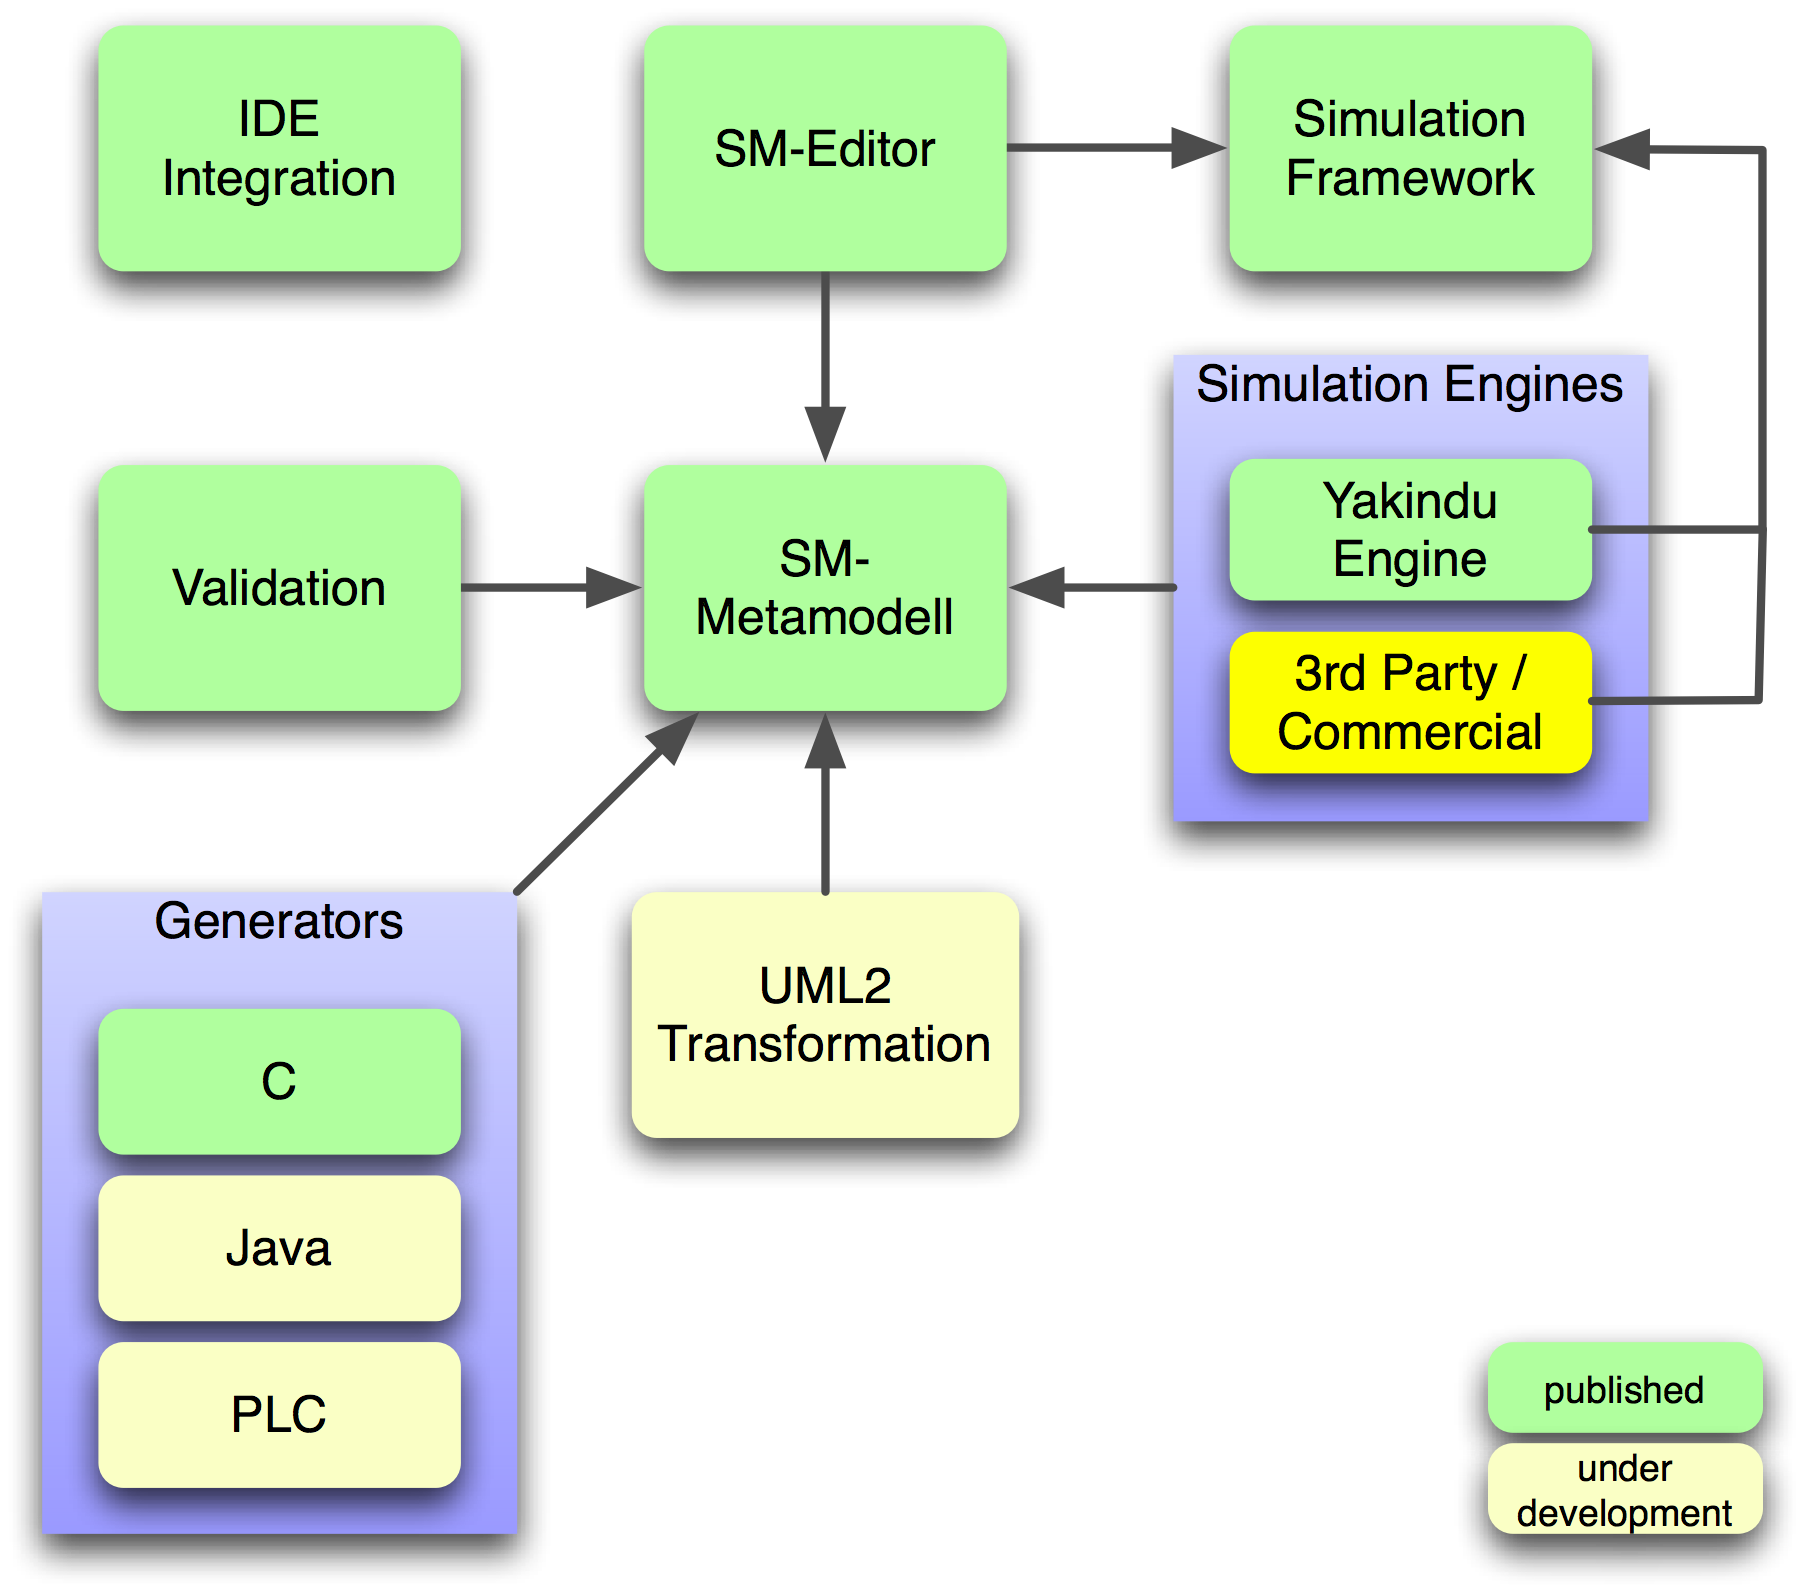
\includegraphics[width=0.7\textwidth]{Pictures/ToolArchitektur}
\caption{\label{fig:toolArchitecture}Tool architecture}
\end{figure}
\clearpage

